% !TeX root = ../../main.tex
\newpage
\section{Generator sztucznych danych}

Generator sztucznych danych został napisany w języku \textit{JavaScript} jako aplikacja internetowa, z prostym i czytelnym interfejsem użytkownika.
Do zbudowania interfejsu wykorzystano bibliotekę \textit{React} \cite{react}.
Ekran aplikacji dzieli się na dwie częsci:
\begin{itemize}
  \item instrukcja objaśniająca jak obsługiwać generator za pomocą klawiatury i myszy;
  \item scena 3D, na której widoczny jest generowany obraz; scena 3D rysowana jest za pomocą biblioteki~\textit{Three.js} \cite{threejs}.
\end{itemize}

\begin{figure}[!htb]
  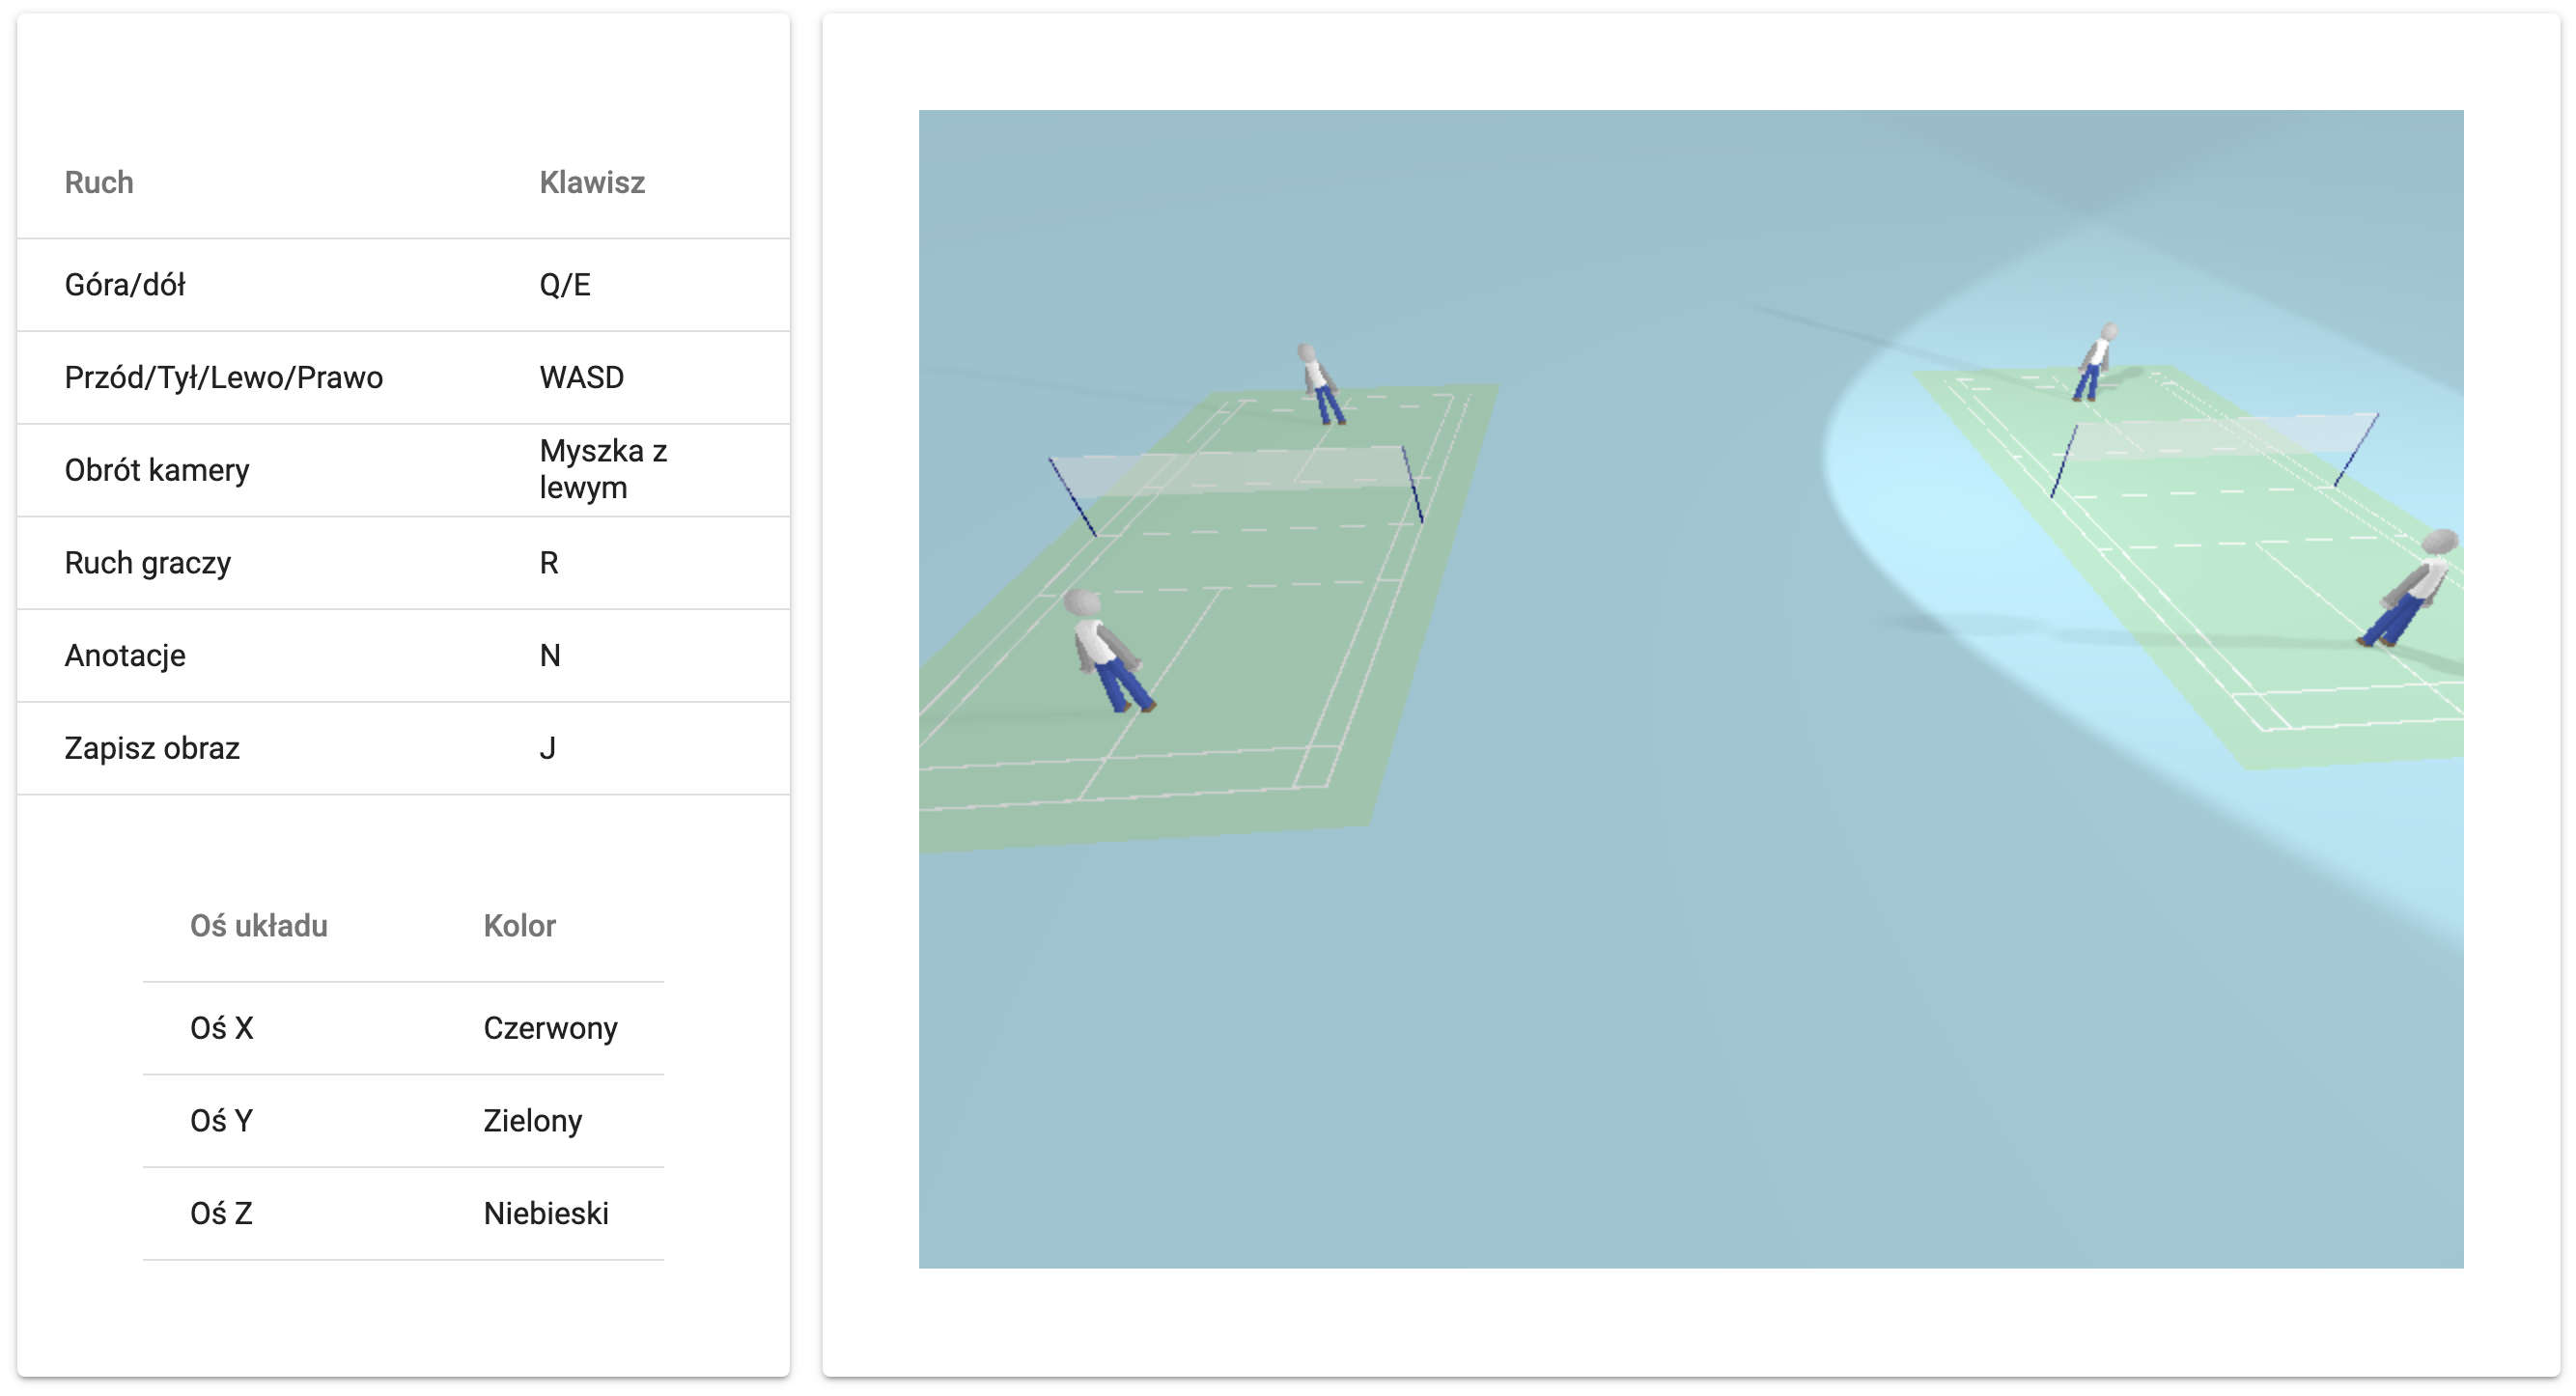
\includegraphics[width=\linewidth]{./generator_3.png}
    \caption{Zrzut ekranu uruchomionego generatora sztucznych danych}
\end{figure}

Interfejs użytkownika pozwala na poruszanie pozycją oraz kierunkiem patrzenia wirtualnej kamery w trójwymiarowej scenie, i zapis rysowanej sceny na dysku. Do tego możliwe jest losowe przemieszczenie zawodników na kortach. Dodatkowe funkcje pomocne w czasie tworzenia generatora służą do pokazania osi wymiarów X, Y i Z w wirtualnej scenie oraz podgląd anotacji obszaru kortów.
